%% ============================================================
%% 片段：s02b-duality   对应原文 PDF 第 14--31 页
%% 本文件由 gw/convert.py 从 arXiv 源码（hep-th/0612073v2）自动生成：
%%   * 公式/编号/引用/图 已经锁定为原文内容，请勿改动任何数学内容与编号；
%%   * 只需把英文正文译为中文，并在每节开头加“本节重点”、关键处加译注。
%% ============================================================


\subsection{电磁对偶}

%% ==== 原文 §2.4：PDF 第 14 页（印刷第 13 页）====
\label{sec:2.4}

${\mathcal N}=4$ 超杨–米尔斯理论具有一个很大的离散对偶对称性群 $\Gamma$。我们乐观地假定，前文描述过的那一类面算符（surface operator）在 $\Gamma$ 的作用下映到自身；在此前提下，我们来确定 $\Gamma$ 如何作用在参数
$(\alpha,\beta,\gamma,\eta)$ 上。


首先考虑基本的电磁对偶（electric-magnetic duality）$S$。
它作用在规范场论的耦合参数 $\tau=\theta/2\pi+4\pi i/g^2$ 上，方式为
$S:\tau\to -1/n_{\mathfrak g}\tau$，其中
当 $G$ 为单边（simply-laced）群时 $n_{\mathfrak g}$ 为 1，否则为 2 或 3
（即 $G$ 的长根与短根长度平方之比）。它同时把 $G$ 映为 $^L\neg G$。那么它如何变换面算符的参数？

\bigskip\noindent{\it $\beta$ 与 $\gamma$ 的变换}

$S$ 对 $\beta$ 与 $\gamma$ 的作用方式非常简单，因为 $\beta$ 与 $\gamma$ 决定了希格斯场特征多项式中的一个极点，而后者在对偶下的变换很简单
（见文献~\cite{ref8} 第 5.4 节；不过我们将采用与那里不同的归一化）。

%
%
由于 $\beta$ 与 $\gamma$ 取值于 $\mathfrak t$，而 $^L\neg\beta$ 与 $^L\neg\gamma$ 取值于 $^L\mathfrak t$，二者之间的比较依赖于从 $\mathfrak t$
到 $^L\mathfrak t$ 的映射的选取。向量空间 $\mathfrak t$ 与 $^L\mathfrak t$ 互为对偶（因此我们也把 $^L\mathfrak t$
记作 $\mathfrak t^\vee$），并且受同一个外尔群作用。
$\mathfrak t$ 上任意外尔不变度量的选取
都给出二者之间一个外尔不变的等同。


为了给第 4 节中几何朗兰兹纲领（geometric Langlands program）的应用做准备，我们将较详细地描述所要采用的等同。\footnote{对规范群
$G_2$ 或 $F_4$，我们即将描述的约定
不同于物理学文献~\cite{ref41,ref42} 中最常见的约定。两种做法之间的关系
在附录 A 末尾说明。另可参见例如文献~\cite{ref71}。} 首先，方便的做法是在 $\mathfrak g$ 上引入一个不变二次型，归一化使短
余根的长度平方为 2。我们把该二次型写作 $(x,y)=-\Tr\,xy$，其中 $x,y\in\mathfrak g$。
（这一记号源于如下事实：当 $G=SU(N)$ 时，$\Tr$ 就是 $N$ 维表示中的迹。）
类似地，我们在 $^L\neg G$ 的李代数 $^L\neg\mathfrak g$ 上引入一个二次型，归一化
使 $G$ 的短根长度平方为 2。我们把它写作 $({}^L\neg x,{}^L\neg y)=
-{}^L\neg\Tr\,^L\neg x{}^L\neg y$。$\mathfrak g$ 上的二次型限制到 $\mathfrak t$ 上，
给出从 $x\in \mathfrak t$ 到 $x^*\in {}^L\mathfrak t$ 的外尔不变映射（满足 $x^*(y)=-\Tr\,xy$）；
同样，$^L\neg\mathfrak g$ 上的二次型限制到 $^L\mathfrak t$ 上，给出外尔不变映射
从 $^L\neg x\in {}^L\mathfrak t$ 到 $^L\neg x^*\in \mathfrak t$。正如附录 A 所解释的，两个映射的复合
等于乘以 $n_{\mathfrak g}$，即

% 式 (2.15)
\setcounter{equation}{14}
\begin{equation}\label{eq:2.15}
  (x^*)^*=n_{\mathfrak g}x,
\end{equation}
 或等价地

% 式 (2.16)
\setcounter{equation}{15}
\begin{equation}\label{eq:2.16}
  ^L\neg\Tr\, x^*y^*=n_{\mathfrak g}\Tr\,xy
\end{equation}

对任意 $x,y\in \mathfrak g$ 成立。此关系在 $G$ 与 $^L\neg G$ 之间是对称的。

现在，如同文献~\cite{ref8} 的式 (2.8) 那样，我们对规范群为 $G$ 的 ${\mathcal N}=4$ 超杨–米尔斯理论
的标量场 $\phi$ 作如下归一化：使其在洛伦兹号差下的动能为

% 式 (2.17)
\setcounter{equation}{16}
\begin{equation}\label{eq:2.17}
  {{\rm Im}\,\tau\over 4\pi}\int d^4x\,\Tr\,D_\mu\phi D^\mu\phi,
\end{equation}

其中 ${\rm Im}\,\tau=4\pi/e^2$。同样，对于规范群为 $^L\neg G$ 的 $S$-对偶理论，我们归一化标量场
$^L\neg \phi$，使其动能为

% 式 (2.18)
\setcounter{equation}{17}
\begin{equation}\label{eq:2.18}
  {{\rm Im}\,{}^L\neg\tau\over 4\pi}\int d^4x\,\Tr\,D_\mu{}^L\neg\phi D^\mu{}^L\neg\phi,
\end{equation}

其中

% 式 (2.19)
\setcounter{equation}{18}
\begin{equation}\label{eq:2.19}
  ^L\neg \tau = -{1\over n_{\mathfrak g}\tau}.
\end{equation}

一般而言，$\phi$ 与 $^L\neg \phi$ 之间不存在局部的等同（只有由这些场构造出的规范不变局部算符之间才可能等同）。然而，为了找出
$\beta$ 与 $\gamma$ 在对偶下如何变换，我们可以像文献~\cite{ref8} 第 5.1 节那样把问题阿贝尔化，
并取一个真空，在其中 $G$ 或 $^L\neg G$ 被标量场的期望值自发破缺到其极大环面（maximal torus）。在这样的阿贝尔真空中，轻标量场
取值于 $\mathfrak t$ 或 $^L\neg \mathfrak t$，而对偶对它们的作用只是一个线性变换，该变换
可以选为外尔不变的（从而是运算 $\phi\to \phi^*$ 的若干倍）。这个变换必须保持
动能，因此

% 式 (2.20)
\setcounter{equation}{19}
\begin{equation}\label{eq:2.20}
  {{\rm Im}\,\tau\over 4\pi}\int d^4x\,\Tr\,D_\mu\phi D^\mu\phi=
 {{\rm Im}\,{}^L\neg\tau\over 4\pi}\int d^4x\,\Tr\,D_\mu{}^L\neg\phi D^\mu{}^L\neg\phi.
\end{equation}

结合式~\eqref{eq:2.19} 与式~\eqref{eq:2.16}，可知在阿贝尔真空中
$\phi$ 与 $^L\neg \phi$ 之间的关系为

% 式 (2.21)
\setcounter{equation}{20}
\begin{equation}\label{eq:2.21}
  ^L\neg \phi= |\tau|\,\phi^*,
\end{equation}

这一关系在 $G$ 与 $^L\neg G$ 之间完全对称，利用式~\eqref{eq:2.15} 与
式~\eqref{eq:2.19} 即可验证。由于 $\beta$ 与 $\gamma$ 刻画 $\phi$ 的奇点，而 $^L\neg\beta$ 与
$^L\neg\gamma$ 同样刻画 ${}^L\neg\phi$ 的奇点，这些参数以同样的方式变换，即 $^L\neg\beta=|\tau|\beta^*$、$^L\neg\gamma=|\tau|\gamma^*$，或者更简洁地

% 式 (2.22)
\setcounter{equation}{21}
\begin{equation}\label{eq:2.22}
  ({}^L\neg\beta,{}^L\neg\gamma)=|\tau|(\beta^*,\gamma^*).
\end{equation}

由于这些参数刻画的是算符而非真空，此公式必定普遍成立，
而不只是在阿贝尔真空中成立。

几何朗兰兹纲领的基本情形可方便地通过令 ${\rm Re}\,\tau=0$ 来研究，
此时式~\eqref{eq:2.22} 可更方便地写成

% 式 (2.23)
\setcounter{equation}{22}
\begin{equation}\label{eq:2.23}
  ({}^L\neg\beta,{}^L\neg\gamma)=({\rm Im}\,\tau)\,(\beta^*,\gamma^*).
\end{equation}

我们也可以把这个关系反解出来：

% 式 (2.24)
\setcounter{equation}{23}
\begin{equation}\label{eq:2.24}
  (\beta,\gamma)=({\rm Im}\,^L\neg\tau)\,({}^L\neg\beta^*,{}^L\neg\gamma^*).
\end{equation}

两式是相容的，因为 $(x^*)^*=n_{\mathfrak g}x$，并且（对虚的 $\tau$）
${\rm Im}\,^L\neg\tau=1/n_{\mathfrak g}\,{\rm Im}\,\tau$。

\begin{yizhu}[原文疑误]以上这句话中的因子关系按定义式~\eqref{eq:2.19} 推不出来。若 $\tau$ 为纯虚，
由 ${}^L\neg\tau=-1/(n_{\mathfrak g}\tau)$ 得 ${\rm Im}\,{}^L\neg\tau=1/(n_{\mathfrak g}\,{\rm Im}\,\tau)$，而不是
$1/n_{\mathfrak g}\cdot{\rm Im}\,\tau$。事实上，只有取 ${\rm Im}\,{}^L\neg\tau=1/(n_{\mathfrak g}\,{\rm Im}\,\tau)$，
式~\eqref{eq:2.23} 与式~\eqref{eq:2.24} 才互相反解（把式~\eqref{eq:2.23} 代入式~\eqref{eq:2.24}，须用到
$({\rm Im}\,\tau)({\rm Im}\,{}^L\neg\tau)n_{\mathfrak g}=1$）。此处照原文保留（PDF 第 16 页），核对时请留意。\end{yizhu}

$\beta$ 与 $\gamma$ 显然不受 $\theta$ 角平移的影响，而正如后文将要讨论的，这一平移
给出对偶群 $\Gamma$ 的第二个生成元 $T:\tau\to\tau+1$。因此它们在 $\Gamma$ 下的完整变换
由式~\eqref{eq:2.22} 确定。若 $G$ 是单边的，结果可以描述得格外简单：此时（正如附录 A 所解释的）
$(\beta,\gamma)$ 与 $(\beta^*,\gamma^*)$ 之间的差别无关紧要。
在这种情况下，式~\eqref{eq:2.22} 连同 $(\beta,\gamma)$ 在 $\tau\to\tau+1$ 下的不变性
蕴含：对一般元素
$\left(\begin{matrix}a&b\\ c&d\end{matrix}\right)\in\Gamma\cong SL(2,\Z)$，变换为 $(\beta,\gamma)\to
|c\tau+d|(\beta,\gamma)$。对任意 $G$ 都可写出类似结果。
若只限于 $\Gamma$ 中把 $G$ 映到自身（而非映到 $^L\neg G$）的指数 2 子群，
式~\eqref{eq:2.22} 则蕴含 $(\beta,\gamma)$ 这一对按一个正因子重新标度。$\Gamma$ 的其他元素
把 $(\beta,\gamma)$ 映为 $(\beta^*,\gamma^*)$ 的正倍数。

\bigskip\noindent{\it $\alpha$ 与 $\eta$ 的变换}

面算符的另外两个参数是 $\alpha\in \TT$ 与 $\eta\in {}^L
\TT$。由于 $S$ 交换 $G$ 与 $^LG$，它也就交换 $\TT$ 与
$^L\TT$，这强烈提示它交换 $\alpha$ 与
$\eta$。这比 $\beta$ 与
$\gamma$ 那种相对平凡的变换有趣得多，也将是本文的基本假设。

事实上，$S^2$ 是对偶群 $\Gamma$ 的中心元素。
它平凡地作用在 $\tau$ 上，而对其他场与
参数则通过电荷共轭作用。所以 $S^2$ 把 $(\alpha,\eta)$
映为 $(-\alpha,-\eta)$。结合 $S$ 交换
$\TT$ 与 $^L\neg\TT$ 这一事实，可知在相差一个符号的意义下，$S$ 必须作用为

% 式 (2.25)
\setcounter{equation}{24}
\begin{equation}\label{eq:2.25}
  S:(\alpha,\eta)\to (\eta,-\alpha).
\end{equation}

由于对偶群 $\Gamma$ 含有中心元素
$S^2$，而后者把 $(\alpha,\eta)$ 这一对变号，
式~\eqref{eq:2.25} 中的整体符号取决于我们究竟怎样把 $S$ 从
上半 $\tau$ 平面的一个对称性提升为
$\Gamma$ 的元素。我们在下文式~\eqref{eq:2.52} 中指定所用的提升。

\begin{yizhu}[原文疑误]
原文此处印作 “eqn.~(4.1)”（PDF 第 17 页），但按上下文，用来指定提升的是本节的式~\eqref{eq:2.52}（$S$、$T$ 的矩阵形式）；而式~\eqref{eq:4.1} 是第 4 节中的 $\omega=(\mathrm{Im}\,\tau)\omega_K$，与此处无关。这应是原文引用编号的笔误。译文按上下文排为式~\eqref{eq:2.52}，特此说明。
\end{yizhu}

\bigskip\noindent{\it 阿贝尔情形}

对非阿贝尔的 $G$，我们无法证明式~\eqref{eq:2.25}，而把它看作
Montonen–Olive 对偶猜想在面算符上的自然推广。\footnote{在某些特殊情形下，由更一般的
弦理论对偶猜想可以推出式~\eqref{eq:2.25}，
其依据是第~\ref{sec:6.4}~节所解释的构造。} 然而在 $G=U(1)$ 的情形，我们
可以直接证明 $S$ 确实如此作用，下面就来解释。我们将沿用
文献~\cite{ref43} 中处理阿贝尔 $S$-对偶的做法
（后者又是仿照二维中处理 $T$-对偶的类似做法
%
%
\cite{ref44,ref45}）。


在阿贝尔规范场论中，规范场局部地是一个实一形式
$A$（我们可以把它看作主
$U(1)$-丛\footnote{$U(1)$ 的李代数是实的，所以主
$U(1)$-丛上的联络局部地自然用一个实一形式表示。（相比之下，若把
$A$ 看作酉复线丛 ${\mathcal L}$ 上的联络，而该线丛来自 $U(1)$ 的一个酉表示，
则我们局部地会用一个虚一形式表示它。）}
${\mathcal R}\to M$ 上的联络），其曲率为 $F=dA$。我们取
作用量为\footnote{为了与物理学文献中以及文献~\cite{ref8} 和本文所用的许多约定
更一致（代价是与 Donaldson 理论中通常使用的约定有些紧张），
我们相对文献~\cite{ref43} 把 $\theta$ 的符号反了过来。其效果是把 $\tau\to -\bar\tau$。}

% 式 (2.26)
\setcounter{equation}{25}
\begin{equation}\label{eq:2.26}
  \begin{aligned}\II&={1\over 8\pi}\int_Md^4x\sqrt
h\left({4\pi\over g^2}F_{mn}F^{mn}-{i\theta\over 2\pi}{1\over
2}\epsilon_{mnpq}F^{mn}F^{pq}\right)\\ &=-{i\over
8\pi}\int_Md^4x\sqrt h\left(\tau F^+_{mn}F^{+\,mn}-\bar\tau
F_{mn}^-F^{-\,mn}\right),\end{aligned}
\end{equation}
 其中 $h$ 是 $M$ 上的一个度量，
$\tau=\theta/2\pi+4\pi i/g^2$，$\epsilon_{mnpq}$ 是 Levi-Civita
反对称张量，而 $F^\pm={1\over 2}(F\pm \star F)$ 是 $F$ 的
自对偶与反自对偶投影。正如文献~\cite{ref43} 所解释的，对任意闭四维流形 $M$，$\II$ 在 $\tau\to\tau+2$ 下
模 $2\pi i\Z$ 不变；若 $M$ 是自旋流形，则在 $\tau\to\tau+1$ 下也不变。量子理论只依赖于作用量
模 $2\pi i\Z$（因为作用量以因子
$\exp(-\II)$ 进入路径积分），所以量子理论具有对称性
$\tau\to\tau+1$ 或 $\tau\to\tau+2$，视 $M$ 而定。




我们这里感兴趣的是更微妙的对称性 $\tau\to -1/\tau$。
首先我们回顾一下在没有
面算符时如何看出这一对称性。我们添加一个二形式场 $\CK$（在
文献~\cite{ref43} 中称为 $G$），并假定它在通常的阿贝尔
规范对称性 $A\to A-d\epsilon$ 下不变（其中 $\epsilon$ 是零形式）。但
我们要求扩大的规范对称性
% 式 (2.27)
\setcounter{equation}{26}
\begin{equation}\label{eq:2.27}
  \begin{aligned}A&\to
A+\cb\\
                                       \CK&\to \CK+d\cb,\end{aligned}
\end{equation}

其中 $\cb$ 是主 $U(1)$-丛 ${\mathcal
T}$ 上的任意联络，$d\cb$ 是它的曲率。（普通的麦克斯韦规范
对称性取 $\cb=-d\epsilon$ 即为此特例。）若 $A$
是主 $U(1)$-丛 ${\mathcal R}$ 上的联络，则
$A+\cb$ 是 ${\mathcal R}\otimes {\mathcal T}$ 上的联络，因此为得到
式~\eqref{eq:2.27} 下的不变性，我们需要对 ${\mathcal R}$ 的所有可能
选择求和。变换~\eqref{eq:2.27} 可以把 $\CK$ 的周期
平移 $2\pi$ 的整数倍；因此，若 $D\subset M$ 是一个
二维闭链，便可有
% 式 (2.28)
\setcounter{equation}{27}
\begin{equation}\label{eq:2.28}
  \int_D\CK\to\int_D\CK+2\pi m,
~~m\in\Z.
\end{equation}




寻找具有不变性~\eqref{eq:2.27} 的拉格朗日量的一个显然办法是
令 $\FF=F-\CK$，并把麦克斯韦拉格朗日量中的 $F$ 处处
换成 $\FF$。但这样得到的理论是平庸的，当然并不等价于麦克斯韦理论。为得到
有意思的东西，我们引入另一个场 $\cv$，它是主
$U(1)$-丛 $\tilde{\mathcal R}$ 上的联络，曲率为 $\CV=d\cv$。我们向
作用量中添加一项
% 式 (2.29)
\setcounter{equation}{28}
\begin{equation}\label{eq:2.29}
  \tilde \II={i\over 8\pi}\int_M d^4x
\sqrt h\epsilon^{mnpq}\CV_{mn}\CK_{pq}={i\over 2\pi}\int_M \CV\wedge
\CK.
\end{equation}
 为验证对称性~\eqref{eq:2.27}，注意若 ${\mathcal T}$ 拓扑平庸，则
联络 $\cb$ 整体地定义为一形式，分部积分表明 $\tilde\II$ 在
$\CK\to \CK+d\cb$ 下不变。我们在
式~\eqref{eq:2.29} 中把系数选得使 $\tilde\II$ 即使在
${\mathcal T}$ 拓扑非平庸时也模 $2\pi i\Z$ 不变。

我们现在定义一个扩充的理论，其场变量为 $\cv,\CK,A$，
作用量为
% 式 (2.30)
\setcounter{equation}{29}
\begin{equation}\label{eq:2.30}
  \hat\II(\cv,\CK,A)={i\over 8\pi}\int
d^4x\sqrt h\left(\epsilon^{mnpq}\CV_{mn}\CK_{pq}-\tau
\FF^+_{mn}\FF^{+\,mn}+\bar\tau \FF_{mn}^-\FF^{-\,mn}\right).
\end{equation}
 由以上所述，$\hat\II$ 在式~\eqref{eq:2.27} 下模
$2\pi i\Z$ 的不变性应当已经清楚。阿贝尔
规范场论 $S$-对偶的证明，来自对这个扩充理论的两种不同研究方式的比较。

一种做法是先对 $\cv$ 作路径积分。
积分中依赖于 $\cv$ 的部分是
% 式 (2.31)
\setcounter{equation}{30}
\begin{equation}\label{eq:2.31}
  \sum_{\tilde{\mathcal R}}\int
D\cv\,\exp\left(-{i\over 2\pi}\int_M \CV\wedge \CK\right)
\end{equation}
 其中
$\CV$ 是 $\cv$ 的曲率。我们必须对 $U(1)$-丛
$\tilde{\mathcal R}$ 求和，并且对每个这样的丛，还要在它上面所有联络构成的空间上积分。该积分
给出一个令 $d\CK=0$ 的 $\delta$ 函数。对丛求和则给出一个 $\delta$
函数，其含义是 $\CK$ 的周期取值于 $2\pi\Z$。
这些条件合起来恰好说明：可以通过变换~\eqref{eq:2.27} 取 $\CK=0$。取
$\CK=0$ 之后，我们便回到原来的阿贝尔规范场论~\eqref{eq:2.26}，
其中 $A$ 是唯一的场变量。

所以，作用量为式~\eqref{eq:2.30} 的扩充理论等价于
耦合参数为 $\tau$ 的原理论。接下来，我们考虑研究同一理论的另一种方式。
我们利用扩大的规范不变性~\eqref{eq:2.27} 取 $A=0$。这样做之后，由于
作用量关于 $\CK$ 二次地依赖而不含 $\CK$ 的任何导数（并且关于 $\CK$ 的二次项
非退化），我们可以通过直接求解欧拉–拉格朗日方程把 $\CK$ 用 $\CV$ 表示出来，从而将它“积掉”。（在文献~\cite{ref43} 中，这一
过程在量子层面有更精确的描述。）
这样我们得到关于 $\CV$ 的作用量，即

% 式 (2.32)
\setcounter{equation}{31}
\begin{equation}\label{eq:2.32}
  -{i\over 8\pi}\int_Md^4x\sqrt
h\left(\left(-{1\over\tau}\right)(\CV^+)^2-\left(-{1\over\bar\tau}\right)(\CV^-)^2\right).
\end{equation}

这就是原来的阿贝尔规范场论，只是把联络
$A$ 换成 $\cv$，并把耦合参数 $\tau$ 换成
$-1/\tau$。所以，比较分析扩充理论
\eqref{eq:2.30} 的这两种方式，就得到了阿贝尔规范场论的
$\tau\to -1/\tau$ 对称性。

现在引入一个面算符，其支撑为
二维流形 $D\subset M$。为简单起见，我们
考虑该面算符具有
$\alpha=0$、$\eta\not=0$ 的特殊情形。这意味着，在底层阿贝尔规范场论的
路径积分中，我们要引入一个因子\footnote{虽然 $\eta$ 是一个角变量，我们
仍把它归一化为取值于 $\R/\Z$ 而不是 $\R/2\pi\Z$，
以避免在 $S$-对偶下的变换中出现看似不自然的 $2\pi$ 因子。
另一种做法是把
$\alpha$、$\beta$、$\gamma$ 的定义乘上一个 $2\pi$ 因子。}
% 式 (2.33)
\setcounter{equation}{32}
\begin{equation}\label{eq:2.33}
  \exp\left(i\eta\int_D{F}\right).
\end{equation}
 这
等价于在作用量中添加一项 $-i\eta\int_DF$。为
把面算符纳入扩充理论，我们把 $F$ 换成 $\FF$，并向
作用量~\eqref{eq:2.30} 添加
% 式 (2.34)
\setcounter{equation}{33}
\begin{equation}\label{eq:2.34}
  -i\eta\int_D
{\FF}=-i\eta\int_M \delta_D\wedge {\FF}
\end{equation}
 这里 $\delta_D$ 是与 $D$ 庞加莱
对偶的二形式 $\delta$ 函数。

额外的一项不依赖于 $\cv$，所以若我们先对 $\cv$ 积分，
便回到带该面算符的阿贝尔规范场论。但如果我们改用
扩大的规范对称性取 $A=0$，然后对 $\CK$ 求解，情况又会如何？
作用量中含有两个关于 $\CK$ 线性的项，它们合并为
% 式 (2.35)
\setcounter{equation}{34}
\begin{equation}\label{eq:2.35}
  {i\over
2\pi}\int_M(\CV-2\pi\eta\delta_D)\wedge \CK.
\end{equation}
 为得到此式，
我们用了式~\eqref{eq:2.29} 与式~\eqref{eq:2.34} 中最后给出的表达式。此外，
作用量的这一部分也是唯一含 $\CV$ 的部分。（
作用量的其余部分关于 $\CK$ 是二次的，且与 $\CV$ 无关。）
所以 $\eta\not=0$ 的效果恰恰是把 $\CV$
换成 $\hat \CV=\CV-2\pi\eta\delta_D$。因此当我们再次积掉
$\CK$ 时，将得到与式~\eqref{eq:2.32} 相同的作用量，只是把 $\CV$
换成 $\hat \CV$：
% 式 (2.36)
\setcounter{equation}{35}
\begin{equation}\label{eq:2.36}
  -{i\over 8\pi}\int_Md^4x\sqrt
h\left(\left(-{1\over\tau}\right)(\hat
\CV^+)^2-\left(-{1\over\bar\tau}\right)(\hat \CV^-)^2\right).
\end{equation}


由于 $\hat \CV$ 中的 $\delta$ 函数项，这个作用量可能
发散。由于作用量关于 $\hat \CV$ 是二次的、
实部正定，使作用量有限的唯一办法是要求
$\CV$ 恰好抵消 $\hat \CV$ 中的 $\delta$ 函数
贡献。于是，对路径积分有贡献的
联络必须满足

% 式 (2.37)
\setcounter{equation}{36}
\begin{equation}\label{eq:2.37}
  \CV=2\pi\eta\delta_D+\dots
\end{equation}
 其中省略号代表
在 $D$ 附近正则的项。但这正是
参数为 $\alpha=\eta$ 的面算符的刻画，
把式~\eqref{eq:2.37} 与式~\eqref{eq:2.5} 比较便应清楚。

于是我们已证明，变换 $S:\tau\to -1/\tau$ 把
参数为 $(\alpha,\eta)=(0,\eta)$ 的面算符映为
参数为 $(\eta,0)$ 的面算符。这是式~\eqref{eq:2.25} 的一个特例。为
得到一般情形，只需把式~\eqref{eq:2.30} 中的 $\FF$ 换成
$\FF-2\pi\alpha\delta_D$，然后重复上述计算。把 $A$
规范固定为零并积掉 $\CK$ 后，便回到一个同类型的作用量，
只是 $\tau$ 换成 $-1/\tau$，并且 $\alpha$ 与 $\eta$ 按式~\eqref{eq:2.25} 交换。

\begin{yizhu}[含糊点拨]作者以“应当已经清楚”一笔带过之处（PDF 第 19 页），实质是两步：其一，对丛 $\tilde{\mathcal R}$ 求和并积掉 $\cv$ 之所以给出两个 $\delta$ 函数（分别强制 $d\CK=0$ 与 $\CK$ 的周期属于 $2\pi\Z$），在量子层面需要文献~\cite{ref43} 的细致处理，这里只是形式论证；其二，非阿贝尔情形毫无证明，式~\eqref{eq:2.25} 纯属猜想，其弦论依据见第~\ref{sec:6.4}~节（把 ${\cal N}=4$ 理论嵌入 IIB 型超弦理论，从而得到面算符）。二维 $T$-对偶的对应推理见文献~\cite{ref44,ref45}。\end{yizhu}


\subsection{\texorpdfstring{$\theta$ 角的平移}{θ 角的平移}}
 %% ==== 原文 §2.5：PDF 第 20 页（印刷第 19 页）====
\label{sec:2.5}

现在回到 $G$ 为单的非阿贝尔规范群的情形。除了
$S:\tau\to -1/n_{\mathfrak g}\tau$（我们已在第~\ref{sec:2.4}~节考虑过）之外，对偶群的
另一个生成元是四维 $\theta$ 角的平移，它通过如下一项
进入四维作用量：

% 式 (2.38)
\setcounter{equation}{37}
\begin{equation}\label{eq:2.38}
  \II_\theta=-i\theta {\mathfrak{N}}
\end{equation}
 其中
% 式 (2.39)
\setcounter{equation}{38}
\begin{equation}\label{eq:2.39}
  {\mathfrak{N}}=-{1\over 8\pi^2}\int_M \Tr\,F\wedge F
\end{equation}
 是瞬子数（instanton number）。
$\Tr$ 是 $\mathfrak g$ 上的负定二次型，满足
当 $x$ 为短余根时 $\Tr\, x^2=-2$。（这一记号源于如下事实：当 $G=SU(N)$ 时，$\Tr$ 是
$N$ 维表示中的迹。）这一归一化保证：
若 $M$ 是不带面算符的闭四维流形，且 $G$ 单连通，则 ${\mathfrak{N}}$ 取整数值。
例如，若 $G=SU(N)$，则 ${\mathfrak{N}}
=-\int_Mc_2(E)$，其中 $c_2$ 是第二陈类。当 ${\mathfrak{N}}$
取整数值时，存在对称性 $T:\theta\to \theta+2\pi$，或
$T:\tau\to\tau+1$。这表达了众所周知的事实：量子场论
只依赖于模 $2\pi i\Z$ 的作用量 $\II$。

若 $G$ 不是单连通的，则 ${\mathfrak{N}}$ 取值于
${{1\over k}}\Z$（对某个整数 $k$），此时我们不用 $T$，
而考虑对称性 $T^k:\tau\to\tau+k$。

为记号简便，假定 $G$ 单连通。我们来研究在存在一个
支撑于二维流形 $D$ 的面算符时，对称性 $T$ 的情形。首先，在
面算符所对应的奇点存在时，我们必须精确地定义
用来定义 ${\mathfrak{N}}$ 的积分是什么意思。该积分有一个
体贡献（bulk contribution），来自对 $D$ 的补集的积分：
% 式 (2.40)
\setcounter{equation}{39}
\begin{equation}\label{eq:2.40}
  {\mathfrak{N}}_0=-{1\over 8\pi^2}\int'_M\Tr\,F\wedge F.
\end{equation}
 符号 $\int'_M$
表示对 $D$ 的补集积分，忽略 $D$ 处可能的 $\delta$ 函数贡献。根据式~\eqref{eq:2.5}，
一旦我们选取丛 $E$ 在 $D$ 上的一个延拓，积分还会有一个 $\delta$ 函数贡献。这个
贡献是
% 式 (2.41)
\setcounter{equation}{40}
\begin{equation}\label{eq:2.41}
  {\mathfrak{N}}'=-{1\over 2\pi}\int_D \Tr
\,\alpha F-{1\over 2}D\cap D\,\Tr\,\alpha^2 .
\end{equation}
  为得到式~\eqref{eq:2.41}
（它对应文献~\cite{ref11} 中的命题 5.7），我们用了如下事实：
$D$ 附近 $F$ 的 $\delta$ 函数贡献是
$2\pi\alpha\delta_D$。我们还用了式~\eqref{eq:2.8}。

和
% 式 (2.42)
\setcounter{equation}{41}
\begin{equation}\label{eq:2.42}
  {\mathfrak{N}}={\mathfrak{N}}_0+{\mathfrak{N}}' =-{1\over
8\pi^2}\int'_M\Tr\,F\wedge F-{1\over 2\pi}\int_D \Tr \,\alpha
F-{1\over 2}D\cap D\,\Tr\,\alpha^2
\end{equation}

 取整数值。然而，${\mathfrak{N}}$ 并不是自然的，意思是说：
它依赖于把 $\alpha$ 从 ${\mathfrak t}/
\Lambda_{\rm cochar}$（它自然取值于此）提升到 $\mathfrak
t$ 的选取。原因很简单：取值整数的不变量
$\int_M c_2(E)$（或 $SU(N)$ 之外其他群的相应类比）并不由 $E$ 在
$M\backslash D$ 上的限制决定，而是依赖于 $E$ 在 $D$ 上延拓方式的选取。
不过，$\mathfrak{N}$ 的整性蕴含：模 $\mathbb{Z}$ 约化后，我们得到

% 式 (2.43)
\setcounter{equation}{42}
\begin{equation}\label{eq:2.43}
  {\mathfrak{N}}_0=-{\mathfrak{N}}'={1\over 2\pi}\int_D \Tr\,\alpha
F+{1\over 2}D\cap D\,\Tr\,\alpha^2~{\rm mod}~\mathbb{Z}.
\end{equation}
 由于 ${\mathfrak{N}}_0$ 不依赖于 $\alpha$ 的提升，式~\eqref{eq:2.43} 的
右端模 $\Z$ 也必如此。我们可以这样验证。
$F$ 在 $D$ 上的限制取值于 ${\mathfrak t}$，而它的
积分 ${\mathfrak{m}}=\int_D F/2\pi$ 是一个“磁荷”，
即格 $\Lambda_{\rm cochar}$ 中的一个元素。这个格
实际上与 $^LG$ 的根格重合（因为我们
假定 $G$ 单连通），换言之，就是 $G$ 的余根格。
由于迹的归一化方式，双线性函数 ${\mathfrak{m}},\,{\mathfrak{m}}'\to \Tr\,{\mathfrak{m}}{\mathfrak{m}}'$ 对这个
格中的 ${\mathfrak{m}},\,{\mathfrak{m}}'$ 取整数值，且当 ${\mathfrak{m}}={\mathfrak{m}}'$ 时取偶整数值。
一旦选定 $E$ 的一个延拓，
$\alpha$ 就取值于 $\mathfrak t$，而 $\mathfrak t$ 等同于
$\Lambda_{\rm cochar} \otimes_{\mathbb{Z}}{\mathbb{R}}$。于是我们可以写

% 式 (2.44)
\setcounter{equation}{43}
\begin{equation}\label{eq:2.44}
  {\mathfrak{N}}'=-\Tr\,\alpha{\mathfrak{m}} -{1\over 2}D\cap
D\,\Tr\,\alpha^2
\end{equation}
 从而
% 式 (2.45)
\setcounter{equation}{44}
\begin{equation}\label{eq:2.45}
  {\mathfrak{N}}_0=\Tr\,\alpha{\mathfrak{m}}+{1\over 2}D\cap D\,\Tr\,\alpha^2~{\rm
mod}~\Z.
\end{equation}
 鉴于迹的整性性质以及式~\eqref{eq:2.10}，这个论断在把 $\alpha$ 平移一个
格向量时不变。

我们希望把 $\II_\theta$ 定义得与丛的延拓选取无关。
唯一显然的办法是舍弃 $D$ 处的 $\delta$ 函数贡献，而令

% 式 (2.46)
\setcounter{equation}{45}
\begin{equation}\label{eq:2.46}
  \II_\theta=-i\theta {\mathfrak{N}}_0.
\end{equation}
 这并不意味着
我们将忽略 $\delta$ 函数贡献。相反，我们将从
第~\ref{sec:2.3}~节引入的二维类 $\theta$ 参数 $\eta$ 那里得到这样的贡献。在
同样的记号下，我们把 $\eta$ 对作用量的贡献取为
% 式 (2.47)
\setcounter{equation}{46}
\begin{equation}\label{eq:2.47}
  \II_\eta=-2\pi i \Tr\,\eta{\mathfrak{m}}-\pi i D\cap
D\,\Tr\,\alpha\eta .
\end{equation}
  项 $\Tr\,\eta{\mathfrak{m}}$ 是类 $\theta$ 角 $\eta$ 所应有的
项。在此基础上，我们添加了一个 $c$ 数项，它只依赖于 $\alpha$ 与 $\eta$，
而不依赖于理论的任何场变量。

因此，作用量的这两部分贡献之和为

% 式 (2.48)
\setcounter{equation}{47}
\begin{equation}\label{eq:2.48}
  \hat \II = \II_\theta+\II_\eta= -i\theta {\mathfrak{N}}_0-2\pi i\Tr\,\eta{\mathfrak{m}}-\pi iD\cap D\, \Tr\,\alpha\eta .
\end{equation}
 到了
这一步，我们可以更充分地论证对 $\II_\theta$ 的定义。向 $\II_\theta$ 加上
$\Tr\,\alpha{\mathfrak{m}}$ 的若干倍
不会产生本质影响，
因为可以靠平移 $\eta$ 来补偿。所以我们不妨就按现在的方式
定义 $\II_\theta$。

下面我们将看到，所作的选择给出一个简单的结论：在
$\theta\to\theta+2\pi$ 下 $\alpha$ 与 $\eta$ 必须如何变换。$ \II_\theta$ 的变化为

% 式 (2.49)
\setcounter{equation}{48}
\begin{equation}\label{eq:2.49}
  \Delta \II_\theta=-2\pi i {\mathfrak{N}}_0=-2\pi
i\Tr\,\alpha{\mathfrak{m}}-\pi i D\cap D\,\Tr\,\alpha^2 ~{\rm mod}~2\pi
i \Z ,
\end{equation}
 这里用了式~\eqref{eq:2.45}。


为使理论具有对称性，$\hat \II$ 必须模
$2\pi i\mathbb{Z}$ 不变。为此，我们令 $T:\theta\to\theta+2\pi$ 作用在
$(\alpha,\eta)$ 上为
% 式 (2.50)
\setcounter{equation}{49}
\begin{equation}\label{eq:2.50}
  \begin{aligned}\eta&\to\eta-\alpha\\
\alpha&\to \alpha.\end{aligned}
\end{equation}
  于是 $\II_\eta$ 的变化
恰好抵消 $\II_\theta$ 的变化（模 $2\pi i\Z$），
$\hat \II$ 保持不变。

我们纳入作用量的常数项 $-\pi i  D\cap D\,\Tr\,\alpha\eta$ 在 $\alpha$ 或 $\eta$ 作格平移时
并不模 $2\pi i$ 不变。然而，这种不变性的破坏与这一项本身一样，
与量子场无关。几何上，这意味着当 $D\cap D$ 非零时，
配分函数不是 $\alpha$ 与 $\eta$ 的复值函数，
而是 $\TT\times
{}^L\neg\TT$ 上某个复线丛的截面。
  当然，也
可以从作用量中略去这个 $c$ 数项，转而
声称对称性 $T:\tau\to\tau+1$ 只在一个
$c$ 数意义下成立。

这一讨论可直接推广到 $G$ 不单连通、瞬子数取值于
${1\over k}\Z$ 的情形。此时考虑对称性 $T^k:\tau\to\tau+k$，
同样的推导表明它作用为

% 式 (2.51)
\setcounter{equation}{50}
\begin{equation}\label{eq:2.51}
  \begin{aligned}\eta&\to\eta-k\alpha\\ \alpha&\to
\alpha.\end{aligned}
\end{equation}


下面把结果~\eqref{eq:2.50} 与先前关于电磁对偶作用的结果~\eqref{eq:2.25}
结合起来。首先考虑 $G$ 自对偶且单边的情形，
此时特别地，对偶群就是 $\Gamma=SL(2,\Z)$。真正具有这些性质的
单李群只有 $E_8$。在这种情况下，
$\Gamma$ 由以下元素生成：
% 式 (2.52)
\setcounter{equation}{51}
\begin{equation}\label{eq:2.52}
  S=\left(\begin{matrix}0&
1\\ -1& 0\end{matrix}\right), ~~~T=\left(\begin{matrix}1&1\\ 0&1\end{matrix}\right).
\end{equation}

式~\eqref{eq:2.25} 与式~\eqref{eq:2.50} 告诉我们，当 ${\mathfrak{M}}$ 取
$S$ 或 $T$ 时，$\alpha$ 与 $\eta$ 在 ${\mathfrak{M}}$ 下的变换为

% 式 (2.53)
\setcounter{equation}{52}
\begin{equation}\label{eq:2.53}
  (\alpha,\eta)\to (\alpha,\eta){\mathfrak{M}}^{-1}.
\end{equation}
 因此
这对任意 ${\mathfrak{M}}\in SL(2,\mathbb{Z})$ 都成立。特别地，
$(\alpha,\eta)$ 这一对在
$SL(2,\Z)$ 下自然地变换；而我们关于 $S$ 与 $T$ 作用的结果虽然动机各自独立，
却彼此相容。

\begin{yizhu}[易错点]这里的矩阵约定极易弄错（PDF 第 24 页）：$(\alpha,\eta)$ 按\emph{行向量}变换，即
$(\alpha,\eta)\to(\alpha,\eta){\mathfrak{M}}^{-1}$；若当作列向量而用 ${\mathfrak{M}}$ 去乘，
则 $S$ 与 $T$ 的角色会互换。可自行核对：$(\alpha,\eta)T^{-1}=(\alpha,\eta-\alpha)$，正对应
式~\eqref{eq:2.50} 的 $\eta\to\eta-\alpha$；$(\alpha,\eta)S^{-1}=(-\eta,\alpha)$，即
$S:(\alpha,\eta)\to(\eta,-\alpha)$。又 $S^2=-1$ 给出 $(-\alpha,-\eta)$，正是电荷共轭，与
式~\eqref{eq:2.25} 前关于“提升”导致整体符号不确定的讨论吻合。另需留意：后文 $SU(2)$、$SO(3)$ 的例证（PDF 第 27 页）直接写出
$T:(\alpha,\eta)\to(\alpha,\eta+\alpha)$，与式~\eqref{eq:2.50} 的 $\eta\to\eta-\alpha$ 符号相反（相当于在那里把 $T$ 换成了 $T^{-1}$）；
原文两处并存，公式均照原文保留，阅读时须先固定一种约定，否则 $\alpha$ 的 $\pm$ 号会整体弄反。\end{yizhu}

对任意单群 $G$，推广如下。首先回忆：电荷取值于
$G$ 的特征格（character lattice）\footnote{在物理学文献的许多地方，这里取的是根格与余根格，
因为理论只在 $\R^{3,1}$ 或 $\R^4$ 上考虑，而物理的电荷与磁荷在那里取值于根格与
余根格。然而，可以用威尔逊算符与 't Hooft 算符作为外源电荷来探测理论，这一事实表明
必定可以把关于对偶的通常讨论精细化到
电荷取值于特征格与余特征格的情形。这里所需的正是这一精细化，粗略地说，因为无论是允许威尔逊与 't Hooft
算符、在一般的四维流形上工作，还是引入本文所考虑的那类面
算符，都会出现同样的拓扑问题。 } $\Lambda_{\rm char}$，
而磁荷取值于余特征格（cocharacter lattice）
$\Lambda_{\rm cochar}$。因此全部电荷取值于
格 $\hat\Lambda=\Lambda_{\rm cochar}\oplus \Lambda_{\rm
char}$，它带有自然的非退化斜配对，因为
$\Lambda_{\rm char}$ 与 $\Lambda_{\rm cochar}$ 互为对偶格。
对偶群 $\Gamma$ 线性地作用在这个格上，保持
斜配对，同时也自然地作用在 $\tau=\theta/2\pi
+4\pi i/g^2$ 上。例如，对 $E_8$ 我们有
$\hat\Lambda=\Lambda_{\rm char}\otimes \Z^2$，其中 $\Z^2$ 是秩二格，
而 $\Gamma=SL(2,\Z)$ 通过它在 $\hat\Lambda$ 上的自然作用。
无论如何，$\Gamma$ 总是作用于全部电荷与磁荷，
从而作用于 $\hat\Lambda$。不过细节稍复杂，
特别是在 $G$ 不是单边时，见文献~\cite{ref41,ref42}。

无论如何，$\Gamma$ 在 $\hat\Lambda$ 上的线性作用
诱导出它在 $\hat\Lambda\otimes_\Z\R$ 上的作用，从而在
$(\hat\Lambda\otimes_\Z\R)/\hat\Lambda$ 上的作用。但
$(\hat\Lambda\otimes_\Z\R)/\hat\Lambda$ 正是 $\TT\times
{}^L\neg\TT$。所以 $\Gamma$ 对电荷的作用决定了
它在 $\TT\times {}^L\neg\TT$ 上的作用，而
$(\alpha,\eta)$ 这一对正取值于此。因此它决定了
$(\alpha,\eta)$ 上的一个自然作用。对任意 $G$，式~\eqref{eq:2.25} 与
式~\eqref{eq:2.50} 的含义是：$\Gamma$ 在 $(\alpha,\eta)$ 上的作用，
恰好是它在电荷与磁荷上的作用所决定的那个自然作用。假设~\eqref{eq:2.25} 断言
这对 $S$ 成立；而对 $T:\tau\to\tau+1$ 它是成立的，因为
式~\eqref{eq:2.50} 的推导实际上与文献~\cite{ref46} 关于
$T:\theta\to\theta+2\pi$ 对电荷作用的计算是近亲。

\begin{yizhu}[易错点]此处“自然作用”的方向值得留意（PDF 第 24--25 页）：$(\alpha,\eta)$ 取值于
$\TT\times{}^L\neg\TT=(\hat\Lambda\otimes_\Z\R)/\hat\Lambda$，其中 $\alpha$ 与磁荷（$\Lambda_{\rm cochar}$）、
$\eta$ 与电荷（$\Lambda_{\rm char}$）相对应。因此 $\Gamma$ 作用在 $(\alpha,\eta)$ 上的是它在电荷格上作用的\emph{转置逆}，
这与式~\eqref{eq:2.53} 中的 ${\mathfrak{M}}^{-1}$ 是同一件事。也正因如此，本文必须用特征格／余特征格
（见上一脚注），而不能用根格／余根格：只有在前者，$\alpha$ 与 $\eta$ 才分别与磁荷、电荷一一对应，$S$ 交换二者才自然。\end{yizhu}

\bigskip\noindent{\it 狄拉克弦}



% [FIGURE 1] 原文 PDF 第 25 页；caption 见下，需翻译
\begin{figure}[htbp]
  \centering
  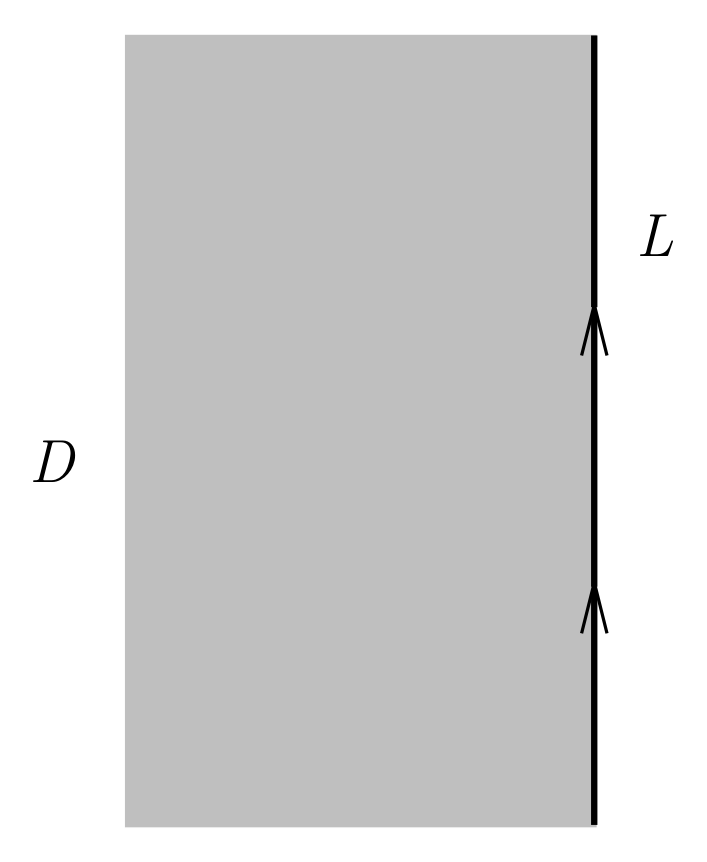
\includegraphics[width=0.62\linewidth]{figures/figure-1.png}
  \caption{一个面算符，其支撑 $D$ 带边界 $L$，而 $L$ 恰是磁单极子或双子的世界线。（原文 Fig.~1，PDF 第 25 页）}
  \label{fig:1}
\end{figure}

现在，把一些细节留给读者，并利用文献~\cite{ref14} 中的一些想法，
我们将对这一结果给出一个非正式的解读。

我们问：面算符的支撑 $D$ 能否像
图~\ref{fig:1} 那样带有边界 $L$？
稍加思考即可看出，若要如此，
$L$ 必须是磁荷为 $\alpha$ 的磁单极子（magnetic monopole）的世界线。绕 $D$ 的规范场和乐必须在边界
$L$ 处解绕，而和乐的这种解绕正是磁荷的特征。

然而，我们并未对磁荷 $\alpha$ 施加狄拉克量子化。既然
我们认为它是在模一个格向量的意义下定义的，那么真正关心的是
狄拉克量子化{\it 不}成立的情形。按照狄拉克的看法，此时为保持规范不变性，
$L$ 必须是通常所谓“狄拉克弦”（Dirac string）的世界体的边界。
在我们的语境中，曲面 $D$ 可以看作该弦的世界体。于是，
我们的面算符可以看作表示与量子化不正确的磁荷
相联系的狄拉克弦。狄拉克用绕弦的规范场单值性来定义狄拉克弦，
所以我们的面算符确实具备成为狄拉克弦世界体的正确性质。

更一般地，若 $\eta\not=0$，
弦末端的磁单极子还带有电荷，因此它是双子（dyon）。

我们关于 $(\alpha,\eta)$ 在 $S$-对偶下像磁荷与电荷一样变换的主张，
可以解读为：与量子化不正确的电荷相联系的狄拉克弦，
在对偶下的变换与正确量子化的电荷完全一样。

\begin{yizhu}[物理图像补充]把 $D$ 视为狄拉克弦世界体的图像与经典磁单极子构造完全平行（PDF 第 25--26 页）。对磁荷不满足
狄拉克量子化条件的磁单极子，必须从它引出一条奇异弦，使绕弦的规范场和乐失去定义；弦的位置并不物理，因为绕过弦一周矢势只差一个规范变换。
本文的面算符恰是把这条“人为”的奇异弦提升为物理算符：支撑 $D$ 就是弦的世界体，端点 $L$ 是磁单极子（或双子）的世界线。
这也说明为何 $\alpha$ 只在模格意义下有定义：把 $\alpha$ 改变一个格向量，只相当于改变丛的延拓，或让一条狄拉克弦穿过曲面。\end{yizhu}

最后给出一个相关的评论，文献~\cite{ref14} 中也有类似的预期。
从物理上说，若把 ${\mathcal N}=4$ 超杨–米尔斯理论
（或任何有兴趣的规范场论，例如标准模型）嵌入到某个在低能下约化为它的更完整的理论中，
面算符就可能出现。嵌入更完整的理论
可能产生在其他语境中所谓的宇宙弦（cosmic string）。假定这样的弦
足够重，以致可以认为它固定在某个位置，并在时空中有一条已知的轨道。
此时就适合考虑在弦存在下的“低能”${\mathcal N}=4$ 动力学。
这将涉及研究 ${\mathcal N}=4$ 理论与某种面算符的耦合。
细节取决于所考虑的具体宇宙弦类型。
产生 Aharonov–Bohm 效应的弦（最早在文献~\cite{ref10} 中探讨）会
导致本文所考虑的那类面算符。在第~\ref{sec:6.4}~节中，我们将考虑一些通过把 ${\mathcal N}=4$ 超杨–米尔斯理论嵌入
更完整的理论（更完整的理论为 IIB 型超弦理论）
而定义的面算符。在宇宙弦理论中，众所周知某些类型的弦可以
断裂，并终止于磁单极子上~\cite{ref47}。


\bigskip\noindent{\it 一个例证}

下面我们更详细地解释在
$G=SU(2)$、$^LG=SO(3)$ 的情形下 $S$-对偶如何作用在电荷上。这将使我们能够
说清楚前面分析中隐含的几点。
沿用文献~\cite{ref48}，我们解释两种不同的
看待该问题的方式。这一讨论在本文其余部分不会用到，
某些地方我们也讲得比较简略。

$SU(2)$ 是单连通的，所以对 $SU(2)$ 规范场论，
瞬子数取整数值，并且存在对称性
$T:\tau\to\tau+1$，其作用如式~\eqref{eq:2.50}。另一方面，对
$SO(3)$，瞬子数取值于 ${1\over 4}\mathbb{Z}$，
若 $M$ 是自旋流形则取值于 ${1\over 2}\mathbb{Z}$。所以 $\theta$ 角的基本
平移对称性是 $T^4:\tau\to\tau+4$，若 $M$ 自旋则为
$T^2:\tau\to\tau+2$。这些对称性的作用如
式~\eqref{eq:2.51}。此外还有对称性 $S:\tau\to -1/\tau$，
它交换 $SU(2)$ 与 $SO(3)$。当 $M$ 非自旋时，$SU(2)$ 规范场论的
对偶对称性群由下式生成：
% 式 (2.54)
\setcounter{equation}{53}
\begin{equation}\label{eq:2.54}
  T=\left(\begin{matrix}1&1\\ 0&1\end{matrix}\right),
~~~ST^4S^{-1}=\left(\begin{matrix}1&0\\-4&1\end{matrix}\right).
\end{equation}
（$ST^4S^{-1}$
是 $SU(2)$ 的对偶对称性，因为 $S^{-1}$ 把 $SU(2)$ 映到
$SO(3)$，$T^4$ 是 $SO(3)$ 的对偶变换，而 $S$
再映回 $SU(2)$。）这个对偶群称为
$\Gamma_0(4)$，是 $SL(2,\Z)$ 的同余子群（congruence subgroup）。它是
$SU(2)$ 规范场论在一般 $M$ 上的对偶对称性群，并且
按式~\eqref{eq:2.53} 作用在 $\alpha$ 与 $\eta$ 上。$SO(3)$ 规范场论的
对偶对称性群同样是 $\Gamma_0(4)$ 的一个拷贝，由 $STS^{-1}$ 与 $T^4$ 生成。
最后当然还有交换这两个群的对称性 $S$。若 $M$ 是自旋流形，则可处处把 4 换成 2，
对偶群同构于 $\Gamma_0(2)$。

$G=SU(2)$ 与 $^LG=SO(3)$ 具有相同的李代数，所以我们可以把
$\TT=\mathfrak t/\Lambda_{\rm rt}$ 与 $^L\neg\TT=\mathfrak t/\Lambda_{\rm wt}$ 看作
同一个空间按不同的格取的商，这两个格分别是
根格与权格（root and weight lattices）$\Lambda_{\rm rt}$ 与 $\Lambda_{\rm wt}$。
$\Lambda_{\rm rt}$ 在 $\Lambda_{\rm wt}$ 中的指数为二。
因此 $\mathfrak t$ 上的恒等映射
投影为从 $\TT$（$\alpha$ 的取值处）到
$^L\neg\TT$（$\eta$ 的取值处）的一个自然的二对一映射。
该映射隐含在变换 $T:(\alpha,\eta)\to
(\alpha,\eta+\alpha)$ 之中。$\mathfrak t$ 上的恒等映射
并不投影为 $^L\neg\TT\to\TT$ 的自然映射，但乘以 2（或任何偶数）的映射
却可以这样投影。于是存在一个自然映射 $ST^2S^{-1}:(\alpha,\eta)\to
(\alpha-2\eta,\eta)$，当 $M$ 是自旋流形时它实现为一个对偶
变换。类似地，运算
$ST^4S^{-1}:(\alpha,\eta)\to (\alpha-4\eta,\eta)$（它对任意 $M$ 都作为对偶变换出现）也是自然定义的。


这种描述方式与物理学文献的说法略有出入，因为那里对
诸如 $SU(2)$ 这样的单边群，对偶群一般被认为是
$SL(2,\Z)$。然而，通常的分析只对 $M=\R^4$ 进行，
且没有仔细考虑威尔逊算符与 't Hooft 算符。在这些
情形下，$SO(3)$ 与 $SU(2)$ 规范场论重合。
可以在 $\R^4$ 上通过添加二维表示中的威尔逊算符来区分这两种理论，以专门指
$SU(2)$；或者添加最小荷的 't Hooft 算符，以专门指
$SO(3)$。（不能同时添加这两类算符，
因为它们彼此不互局域。）如果按这种方式对 $SU(2)$ 与 $SO(3)$
理论加以细化，那么在 $\R^4$ 上合适的对偶群，恰恰就是
我们刚才在一般自旋流形上描述的那些。


其实，这个问题还有另一种表述，我们只给出其梗概，但它确实提供更多信息，
并且其中完整的群 $SL(2,\Z)$ 发挥作用。在这种
做法中，我们总把规范群取为伴随群
$SO(3)$（而不是它的覆盖群 $SU(2)$），但我们指定丛 $E$ 的
第二 Stieffel–Whitney 类 $\xi=w_2(E)$。对具有固定 $\xi$ 的所有 $SO(3)$-丛求和，我们为每个 $\xi$ 定义一个
配分函数\footnote{连同构成一个量子场论的一整套算符、关联函数、
量子态、膜等等。在更完整的描述中，被 $SL(2,\Z)$ 变换的是整个量子场论，
而不仅仅是这组配分函数。} $Z_\xi(\tau)$。然后可以证明
\cite{ref48}，$Z_\xi(\tau)$ 在一个 $SL(2,\Z)$ 的酉
表示中变换。

要把参数为 $\alpha,\eta$、支撑在曲面 $D$ 上的面算符
纳入这种做法，人们定义
$\alpha$ 与 $\eta$ 取值于 $\TT$，即单连通群 $SU(2)$ 的极大环面。于是对每个 $\xi$ 我们有一个
配分函数 $Z_\xi(\tau;\alpha,\eta)$，而主张是：
这一族配分函数按 $SL(2,\Z)$ 的一个表示变换（$SL(2,\Z)$ 以通常方式作用在 $\tau$ 上，
按文献~\cite{ref48} 所述作用在 $\xi$ 上，并按
式~\eqref{eq:2.53} 所述的自然作用，作用于 $\alpha$ 与
$\eta$ 上）。

用参数 $\xi,\alpha,\eta$ 来描述略有冗余。为说明这种
冗余，我们对极大环面 $\TT$（$\alpha$ 与 $\eta$ 的取值处）采用乘法记号，
并回忆这个环面含有 $SU(2)$ 中心的元素 $-1$。于是把 $\alpha$ 变为 $-\alpha$ 等价于按式~\eqref{eq:2.6} 把 $\xi$ 换成
$\xi+[D]$；而把 $\eta$ 变为 $-\eta$ 则使配分函数
$Z_\xi(\tau;\alpha,\eta)$ 乘以 $(-1)^{(\xi,D)}$（这一点在第~\ref{sec:4.2}~节末尾
有实质性的说明）。这种冗余与 $SL(2,\Z)$ 的作用相容，
但若不想让 $SL(2,\Z)$ 的作用显得更不自然，似乎很难把它消除。

\subsection{列维子群与更一般的面算符}

%% ==== 原文 §2.6：PDF 第 28 页（印刷第 27 页）====
\label{sec:2.6}

下面描述面算符定义的一个简单而重要的推广：把
极大环面 $\TT$ 换成 $G$ 的某个包含 $\TT$ 的更一般的子群 $\mathbb{L}$。
我们还假定 $\mathbb{L}$ 可以刻画为 $G$ 中与某个 $\alpha\in \mathfrak t$ 交换的子群。
这样的 $\mathbb{L}$ 称为 $G$ 的列维型子群（subgroup of Levi type）。
若两个这样的群在 $G$ 中共轭，就认为它们等价。
通常的情形是 $\alpha\not= 0$ 且 $\mathbb{L}$ 是 $G$ 的真子群，但我们也会
考虑 $\alpha=0$、$\mathbb{L}=G$ 的情形。任何列维子群（Levi subgroup）都包含 $\TT$，所以 $\TT$ 是极小列维子群。
非极小列维子群的一个典型例子是 $SU(3)$ 中如下形式的子群：

% 式 (2.55)
\setcounter{equation}{54}
\begin{equation}\label{eq:2.55}
  \left(\begin{matrix}* & * & 0 \\
                        * & * & 0 \\
                        0 & 0 & * \end{matrix}\right).
\end{equation}

它与 $U(2)$ 同构，实际上是一个次极小列维子群，因为
更小的列维子群只能是 $\TT$ 本身。一般地，对秩为 $r$ 的任意 $G$，
次极小列维子群同构于 $SU(2)\times U(1)^{r-1}$
或它对 $\Z_2$ 的商。

现在我们来定义所谓的 $\mathbb{L}$ 型面算符。按这种说法，
我们最初定义的面算符是 $\TT$ 型算符；我们也称它
为一般面算符。为定义 $\mathbb{L}$ 型面算符，我们考虑一个二维流形 $D$，其上带有
经典层面由通常参数 $(\alpha,\beta,\gamma)$ 标记的规范场论奇点。但
现在要求这些参数是 $\mathbb{L}$ 不变的。此外，当我们做量子
路径积分时，所除掉的规范变换是那些限制到 $D$ 上取值于 $\mathbb{L}$ 的变换，
而不只是取值于 $\TT$ 的那些。
正是由于最后这一步，$\mathbb{L}$ 型面算符才不只是我们最初
所定义的面算符（即 $(\alpha,\beta,
\gamma)$ 单纯取值于 $\mathfrak t$ 的 $\TT$ 型算符）在参数
为 $\mathbb{L}$ 不变时的特例。$\mathbb{L}$ 型面算符
是新东西，对应于不同的路径积分。事实上，我们将在第~\ref{sec:3.6}~节看到，若 $\mathbb{L}$ 以 $\TT$
为真子群，则当参数变为 $\mathbb{L}$ 不变时，$\TT$ 型面算符
会变得奇异。所以对于这类特殊参数，真正有意义的算符
是新的 $\mathbb{L}$ 型面算符。


在量子层面，还有一个额外的参数 $\eta$，即第~\ref{sec:2.3}~节的二维
$\theta$ 角 $\eta$。在当前情形下，群 $\TT$ 被 $\mathbb{L}$ 取代，
$\eta$ 不是取值于 $^L\neg \TT$，而是取值于某个子群。
事实上，我们希望把 $\eta$ 定义为 $\mathbb{L}$ 的阿贝尔部分的 $\theta$ 角。
为方便描述 $\eta$ 的取值，注意到列维子群 $\mathbb{L}\subset G$ 与
列维子群 $^L\neg \mathbb{L}\subset{} ^L\neg G$ 之间存在自然的对应。
描述这一对应的一种方式是：利用 $G$ 的外尔群 ${\mathcal W}$ 与
$^L\neg G$ 的外尔群 $^L\neg{\mathcal W}$ 自然等同这一事实。（见附录 A。）
此外，$\mathbb{L}$ 与 $^L\neg\mathbb{L}$
的外尔群分别是 ${\mathcal W}$ 与 $^L\neg {\mathcal W}$ 的子群。$\mathbb{L}$ 与 $^L\neg\mathbb{L}$ 之间的
对应简单说来就是它们有相同的外尔群，我们
把它记作 ${\mathcal W}_\mathbb{L}$。
表述 $\mathbb{L}$ 与 $^L\neg \mathbb{L}$ 之间对应的另一种说法是：$^L\neg \mathbb{L}$ 的余根
（它们是 $^L\neg G$ 的余根的子集）是 $\mathbb{L}$ 的余根的倍数——长余根与短余根
所乘的倍数不同。在明确了这些之后，
$\mathbb{L}$ 型面算符依赖于参数 $(\alpha,\beta,\gamma,\eta)$，它们
取值于 $\TT\times \mathfrak t\times \mathfrak t\times {}^L\neg
\TT$ 的 ${\mathcal W}_\mathbb{L}$ 不变部分。我们在这里用到了
如下事实：$(\alpha,\beta,\gamma)$ 的 $\mathbb{L}$ 不变性等价于
${\mathcal W}_\mathbb{L}$ 不变性。用 ${\mathcal W}_\mathbb{L}$ 不变性来表述有一个重要的
优点：它使我们能把 $\eta$ 与其他变量同等对待。
这比说 $(\alpha,\beta,\gamma)$ 是 $\mathbb{L}$ 不变的、
而 $\eta$ 是 $^L\neg \mathbb{L}$ 不变的要好。要求 $\eta$ 必须
为 ${\mathcal W}_\mathbb{L}$ 不变是正确的，因为这意味着 $\eta$ 是
限制在 $D$ 上的规范丛 $E$ 的阿贝尔磁通量的一个特征；
该丛的结构群是 $\mathbb{L}$，而它的特征类是
${\mathcal W}_\mathbb{L}$ 不变的。

我们把第~\ref{sec:2.4}~节的对偶猜想推广为：$\mathbb{L}$ 型面算符
在对偶下映为 $^L\neg \mathbb{L}$ 型面算符，参数
按熟悉的方式变换：$(\alpha,\beta,\gamma,\eta)\to(\eta,\beta,\gamma,-\alpha)$。


\bigskip\noindent{\it 更多群论}

下面描述一些在本文其余部分会用到的群论。

列维子群与所谓 $G_\C$ 的抛物子群密切相关。
取一个 $\alpha\in \mathfrak t$，使得与它交换的元素恰好组成 $\mathbb{L}$。我们说
这样的 $\alpha$ 是 $\mathbb{L}$-正则的（若 $\mathbb{L}=\TT$，就简单地说 $\alpha$ 是正则的）。
令 $\EUP$ 为 $G_\C$ 中李代数为 $\mathfrak p$ 的子群，
$\mathfrak p$ 由满足下式的元素 $\psi\in \mathfrak g$ 张成：
% 式 (2.56)
\setcounter{equation}{55}
\begin{equation}\label{eq:2.56}
  [\alpha,\psi]=i\lambda\psi,
~\lambda\geq 0.
\end{equation}
  这种形式的群称为 $G_\C$ 的抛物子群（parabolic subgroup）。
若在式~\eqref{eq:2.56} 中把条件 $\lambda\geq 0$ 换成 $\lambda>0$，我们便得到
子群 $\EUN\subset \EUP$ 的李代数
$\mathfrak n$，$\EUN$ 称为 $\EUP$ 的幂幺根（unipotent radical）。



例如，对 $G_\C=SL(3,\C)$ 与
$\mathbb{L}=\TT$，可以取 $\alpha=i\,{\rm diag}(y_1,y_2,y_3)$，其中 $y_i$ 为实数
且 $y_1>y_2>y_3$。此时得到的抛物群是上三角
矩阵构成的群

% 式 (2.57)
\setcounter{equation}{56}
\begin{equation}\label{eq:2.57}
  \left(\begin{matrix}*&*&*\\ 0&*&*\\ 0&0&*\end{matrix}\right),
\end{equation}

它称为博雷尔子群（Borel subgroup）$\EUB$。在这个例子中，幂幺根 $\EUN$
由如下形式的矩阵组成：

% 式 (2.58)
\setcounter{equation}{57}
\begin{equation}\label{eq:2.58}
  \left(\begin{matrix}1&*&*\\ 0&1&*\\ 0&0&1\end{matrix}\right),
\end{equation}


用外尔变换置换特征值，会得到另一个不同于我们所取的 $\TT$-正则（或简称正则）
$\alpha$。这导致一个外尔共轭的博雷尔
子群 $\EUB'$。
更一般地，对任意 $G$，
与序对 $(\TT,\alpha)$ 相联系的抛物子群
称为博雷尔子群 $\EUB$，它在外尔变换下唯一。
$\EUB$ 是极小抛物子群，正如 $\TT$ 是极小列维子群。

非极小列维子群 $\mathbb{L}$ 可能联系着若干个不等价的抛物子群。
例如，在式~\eqref{eq:2.55} 的例子中，我们可以取

% 式 (2.59)
\setcounter{equation}{58}
\begin{equation}\label{eq:2.59}
  \alpha=iy\left(\begin{matrix}1&0&0\\ 0&1&0\\ 0&0&-2\end{matrix}\right),
\end{equation}

其中 $y$ 为非零实数。若 $y$ 为正，得到由如下形式的矩阵
构成的抛物子群 $\EUP$：

% 式 (2.60)
\setcounter{equation}{59}
\begin{equation}\label{eq:2.60}
  \left(\begin{matrix}*& * & * \\
                        * & * & * \\
                        0 & 0 & * \end{matrix}\right),
\end{equation}
但若 $y$ 为负，则得到不等价的抛物子群 $\EUP'$，
                        它由如下形式的矩阵构成：

% 式 (2.61)
\setcounter{equation}{60}
\begin{equation}\label{eq:2.61}
  \left(\begin{matrix}* & * & 0 \\
                        * & * & 0\\
                        * & * & * \end{matrix}\right).
\end{equation}

幂幺根 $\EUN$ 与 $\EUN'$ 由如下形式的矩阵组成：

% 式 (2.62)
\setcounter{equation}{61}
\begin{equation}\label{eq:2.62}
  \left(\begin{matrix}1 & 0 & * \\
                        0 & 1 & * \\
                        0 & 0 & 1 \end{matrix}\right),
\end{equation}

或

% 式 (2.63)
\setcounter{equation}{62}
\begin{equation}\label{eq:2.63}
  \left(\begin{matrix}1 & 0 & 0 \\
                        0 & 1 & 0 \\
                        * & * & 1 \end{matrix}\right).
\end{equation}

\begin{yizhu}[易错点]式~\eqref{eq:2.59} 中 $\alpha$ 的正负给出\emph{不同}的抛物子群（PDF 第 30 页）：$\alpha$ 与 $-\alpha$ 分别对应彼此不共轭的
$\EUP$ 与 $\EUP'$（形状见式~\eqref{eq:2.60} 与式~\eqref{eq:2.61}），但两者的列维部分相同，都是式~\eqref{eq:2.55} 中的 $\mathbb{L}$。
所以“非极小列维子群联系着若干不等价的抛物子群”说的是：列维子群只固定块对角部分，而上三角或下三角的取向由 $\alpha$ 的指向（即 $(\TT,\alpha)$ 中的 $\alpha$）另行选定；
取 $\alpha=0$ 则退化为 $\mathbb{L}=G$、$\EUP=G_\C$ 的极大情形。\end{yizhu}

\bigskip\noindent{\it 极大列维子群}

若 $\alpha=0$，便得到上述构造的一个特殊情形：$\mathbb{L}=G$、$\EUP=G_\C$、
$\EUN=1$。最方便的做法是允许这一特殊情形，并把 $G$ 本身
看作一个极大列维子群。

在上面的讨论中，我们对 $\alpha$ 与 $\eta$ 是取值于李代数还是取值于环面
这一点略欠精确。取值于环面的情形给出更一般的构造，因为
${\mathcal W}_\mathbb{L}$ 不变的 $\alpha$ 或 $\eta$ 构成的空间可能不连通。我们针对
$\mathbb{L}=G$ 的情形把这一点说清楚。
$\alpha$ 为 $G$ 不变的条件表明它取值于 $G$ 的中心，我们
把它记作 ${\mathcal Z}(G)$。于是，支撑在曲面 $D$ 上的 $G$ 型面算符
的含义是：规范场定义在 $M\backslash D$ 上，
并且绕 $D$ 的单值性由指定的元素
$\alpha\in {\mathcal Z}(G)$ 标记。与选择 $\alpha$ 相对偶的是：
$D$ 上的 $G$-丛在拓扑上由一个特征类
$\xi\in H^2(D,\pi_1(G))\cong
\pi_1(G)$ 分类，而路径积分可以按取值于 ${\rm Hom}(\pi_1(G),U(1))$ 的离散 $\eta$ 角的选择
来加权。有限群 ${\mathcal Z}(G)$ 与 ${\rm Hom}(\pi_1(G),U(1))$ 在对偶下互换，
而自然的对偶猜想是：$\alpha$ 与 $\eta$ 的离散版本
按通常方式互换。

\begin{yizhu}[易错点]极大列维子群（$\mathbb{L}=G$，PDF 第 31 页）情形下，$\alpha$ 不再是李代数向量，而是中心里的离散元素
$\alpha\in{\mathcal Z}(G)$；$\eta$ 也变成取值于有限群 ${\rm Hom}(\pi_1(G),U(1))$ 的离散 $\theta$ 角。
原文指出，这两个有限群在对偶下互换，这正是式~\eqref{eq:2.25} 中 $S$ 交换 $\alpha,\eta$ 的离散版本。
注意不可把这一情形当作 §2.4--§2.5 环面取值情形的平凡极限：此处单值性取在中心里，反映的是 $G$-丛一般无法延拓过 $D$，
其障碍正是特征类 $\xi\in H^2(D,\pi_1(G))$。\end{yizhu}

虽然我们关于 $\mathbb{L}$ 型面算符的对偶猜想意在
涵盖这些不连通分支，本文不会详细
讨论它们。
